\documentclass[12pt]{article}
\usepackage{graphicx}
\usepackage{xcolor}
\usepackage{subfigure}
\usepackage[margin=1.0in]{geometry}
\usepackage{float}
\usepackage{ulem}
\usepackage{amsmath}
\usepackage{mathtools}
\usepackage{wrapfig}
\renewcommand{\baselinestretch}{1.5}
\usepackage[utf8]{inputenc}
\author{Shivesh Pathak}
\title{Developing effective theories for the square lattice Hubbard model using density matrix downfolding}

\begin{document}
\maketitle
\begin{abstract}
A core problem of condensed matter physics is understanding how to systematically develop low-energy effective models for strongly correlated electron systems. 
We believe that a density matrix downfolding (DMD) method can be used to systematically build effective theories for such systems beginning with a high energy theory like the \textit{ab-initio} Hamiltonian H$_\text{ab}$.
We present as a preliminary result an effective theory developed using DMD which can accurately reproduce the spectra and properties of the lowest lying excitations of the CuO molecule.
As a step towards bulk strongly correlated materials, we propose developing effective theories using DMD for the simplest toy system which exhibits strongly correlated behavior: the 1-band square lattice Hubbard model at half-filling for various couplings U and temperatures T.
\end{abstract}
Committee: Lucas Wagner, ...
\pagebreak

\section{Introduction}
A core problem of condensed matter physics is understanding how to systematically develop low-energy effective models for strongly correlated electron systems. 
In the forefront of modern research are materials like high temperature superconductors and heavy fermion systems for which simple effective theories have not yet been found. 
For example, the cuprate family of high-Tc superconductors have an intricate phase diagram in the doping-temperature space  with a robust anti-ferromagnetic (AFM) charge-transfer insulator state near zero doping, a prominent superconducting dome in the 0.1 - 0.2 hole doped region at low temperatures with psuedo-gap and non-Fermi liquid metallic phases at higher temperatures and Fermi liquid like behavior in the overdoped area, of which only the AFM insulating and Fermi liquid phases have well understood mechanism and models. 
The iron-pnictides also have superconducting domes, non-Fermi liquid like metallic phases, a spin-density-wave antiferommagnetic phase, all under various dopings and temperatures. 
Heavy-fermion materials have a purported quantum critical point between an AFM and Fermi-liquid phase which houses a superconducting dome, leading to another phase diagram for which building model Hamiltonians is very challenging. 

The fundamental barrier in writing down low-energy theories for strong correlated materials is the existence of non-perturbative interactions between various degrees of freedom - for example, lattice, spin and charge. 
Consider just the cuprate case for now, the two phases which are relatively well understood contain a singular important degree of freedom in the low-energy space. 
Near zero doping the cuprates are charge-transfer insulators with localized spin-1/2 low-energy degrees of freedom and resemble a Heisenberg antiferromagnet away from the magnetic Brillouin zone. 
In the heavily overdoped side, the lowest energy single-particle excitations look like well defined quasiparticles resembling a Fermi liquid apart from non-standard plasmonic modes. 
In the intermediate doping region where the low-energy excitations cannot be easily sectioned into spin-like or electron-like only, we see the emergence of exotic phases and where most difficulties arise in writing down low-energy effective models. 
On top of that, this entire discussion did not include any lattice effects like structural phase transitions which many strongly-correlated materials have as well.

Common approaches to building suitable model Hamiltonians for strongly correlated materials involve using single particle theories like density functional theory (DFT).
One-body terms are typically obtained by projecting the solutions from the DFT band structure onto a localized single-particle basis, giving an estimate of hoppings and occupations on a lattice model.
Two-body terms in the model are developed by assuming a screened Coulomb interaction based on constrained DFT or RPA.
Aside from this method, L\''{o}wdin methods coupled to a stochastic method and canonical transformations have also been used to develop effective theories.
These methods have the drawback that the constructed effective theory typically does not come with any estimate of the quality of the model, therefore making model validation a phenomenological task which can lead to unclear biases in the model construction.

We propose using a density matrix downfolding (DMD) procedure to systematically develop low-energy effective theories of the 1-band nearest-neighbor Hubbard model on a square lattice for various couplings U and temperatures T at half-filling as a stepping stone towards building effective theories for strongly correlated materials. 
The Hubbard model is a simple model with nearest-neighbor hopping and a local on-site Coulomb repulsion, parameterized by a single ratio U/t: 
\begin{equation}
H_\text{hub} = -t \sum_{\langle i,j \rangle,\sigma}( c_{i^\dagger,\sigma} c_{j,\sigma} + h.c.) + U \sum_i n_{i\uparrow} n_{i\downarrow}
\label{hubbard}.
\end{equation}
The solutions in 1-d are well understood via the Bethe ansatz, however, the 2-d square lattice Hubbard model has no known exact solution.  
A few well accepted facts do exist for this model, such as the existence of long-range anti-ferromagnetic (AFM) order for any U$>$0 at T = 0 and a Mott-Heisenberg limit as $U/t \rightarrow \infty$ at low temperatures.
The T = 0 diagram of the model at half-filling has been a long-standing source of controversy between two groups:  those who believe that for any U $>$ 0 the model exhibits Mott-Heisenberg behavior, and those who believe that there is a transition at finite U$^*$ between Slater and Mott-Heisenberg behavior.
While recent numerical and theoretical calculations tend to agree with the latter position, non-negligible evidence for the prior does exist. 
Further, modern finite temperature calculations indicate thermal transitions in the weak to moderate coupling region between the Slater phase at T = 0, pseudogap phase below T$_{pg}$ and a Fermi liquid phase above.
A finite temperature psuedogap to Mott insulator transition has also been found between the weak to strong coupling limits.
The nature of these transitions as phase transitions or simply crossovers is poorly understood.
The relative simplicity of the half-filled Hubbard model, potential complexity of its phase diagram in U-T space,  and the lack of well-established low-energy theories for moderate U/t lends the model as a useful playground for our new downfolding procedure in preparation for tackling realistic strongly correlated electron systems. 

The DMD procedure allows us to systematically develop low-energy effective theories for any Hamiltonian and Hilbert space $(H, \mathcal{H})$.
The procedure defines a method for downfolding the \textit{ab-initio} energy functional and Hilbert space onto an effective energy functional defined on a low-energy subspace of the Hilbert space 
\begin{equation}
(E, \mathcal{H}) \xrightarrow{\text{DMD}} (E_\text{eff}, \mathcal{LE} \subset \mathcal{H}), \text{ s.t. }
\forall |\Psi\rangle \in \mathcal{LE}, \ E_\text{eff}[\Psi] - E[\Psi] = \epsilon[\Psi] + E_0.
\label{eq:DMD}
\end{equation} 
The energy functionals can be written as expectations over Hamiltonian operators $E = \langle \Psi | \hat{H} |\Psi \rangle$, $E_\text{eff} = \langle \Psi | \hat{H}_\text{eff} |\Psi \rangle$, $\epsilon$ represents the error in our effective theory, and $E_0$ is a constant energy shift.
Broadly the DMD method consists of four steps which will be discussed in detail later: 
A) Defining the space of low-energy excitations which $E_\text{eff}$ should be able to describe accurately.
B) Sampling, at minimum, a set of states in $\mathcal{H}$ which probe the chosen low-energy excitations in a statistically independent manner. The selected states need not be eigenstates. 
C) Constructing a set of candidate models which are linear in reduced density matrix (RDM) descriptors with variable coefficients $\{c\}$
\begin{equation}
E_\text{eff} = \sum_k c_k \langle \Psi | \hat{d}_k |\Psi \rangle + E_0.
\label{eq:Eeff}
\end{equation}
Here $\hat{d}_k$ are Hermitian operators typically composed of 1- or 2-RDM elements. 
Examples of possible $\hat{d}_k$ are number operators $\hat{n}_i$ and exchange operators $\vec{S}_i \cdot \vec{S}_j$.
Additionally, a single particle basis must be built to express RDM elements on and should be chosen such that variations among states in $\mathcal{LE}$ are mostly described by variations in the projection of these states onto the basis.
D) Using the samples to fit the coefficients $\{c\}$ by linear regression such that $E_\text{eff}$ satisfies the conditions in \eqref{eq:DMD} with the smallest error $\epsilon$ possible. 
The fitting procedure is typically an ordinary linear regression, however, one may use a custom cost function in the regression as well. 
In order to conduct the linear regression for a functional like \eqref{eq:Eeff}, one needs to calculate for each state sampled from $\mathcal{LE}$ the expectation values of $\hat{H}$ and every descriptor $\{\hat{d}_k\}$ used in the regression.
In principle, if conducted with no approximations, the DMD method is rigorously guaranteed to obtain exact results, namely $\epsilon[\Psi] = 0$.
For real world systems we will work with $H = H_\text{ab}$, the \textit{ab-initio} Hamiltonian under the Born-Oppenheimer approximation with psuedopotentials:
\begin{equation}
\hat{H}_\text{ab} = -\frac{1}{2} \sum_{i} \nabla_i^2 - \sum_{i,I}\frac{Z}{|r_i - R_I|} + \sum_{i<j}\frac{1}{|r_i - r_j|}
\label{eq:Hab}
\end{equation}
where $i$ indicates electrons and $I$ nuclei, and the unit of energy is Hartree (Ha).

When downfolding $\hat{H}_\text{ab}$ we will use fixed-node diffusion Monte Carlo (FN-DMC) to access states in $\mathcal{LE}$ and accurately calculate their \textit{ab-initio} energies and RDM elements.
Diffusion Monte Carlo (DMC) is a quantum Monte Carlo method which projects out the ground state of a Hamiltonian given some initial trial wave function.
Consider a trial wave function $|\Psi_T\rangle$ and the Hamiltonian $\hat{H}_\text{ab}$ with ground state $|\Phi_0\rangle$. We apply the projector $e^{-\tau \hat{H}_\text{ab}}$ as $\tau \rightarrow \infty$ to $|\Psi_T \rangle$
\begin{equation}
\lim_{\tau \rightarrow \infty} e^{-\tau \hat{H}_\text{ab}} |\Psi_T\rangle 
\equiv \lim_{\tau \rightarrow \infty} |\Psi_\text{DMC}(\tau)\rangle \propto \langle \Phi_0|\Psi_T\rangle |\Phi_0\rangle,
\end{equation}
projecting out the ground state as long as the trial wave function we choose is not orthogonal to the ground state. 
The stochastic implementation involves moving samples from the trial function $\Psi_T(R)$ using the Green function $G(R, R^\prime, \tau) = \langle R | e^{-\tau(\hat{H}_\text{ab} - E_T)} | R^\prime \rangle$. Since $H_\text{ab} = T + V$, kinetic and potential energy terms, the Green function is approximated by a Trotter expansion $G(R, R^\prime, \tau) = \langle R | e^{-\tau(\hat{H} - E_T)} | R^\prime \rangle \sim \Big[e^{-d\tau(V(R) + V(R^\prime))/2} \langle R| e^{-d\tau(\hat{T} - E_T)}|R^\prime \rangle + O(d\tau^2) \Big]^N $ where $d\tau = \tau/N$.
This expansion can be interpreted as an interative procedure where samples are moved N times with a small timestep $d\tau$ until convergence.
The constant $E_T$ is a trial energy used to control the normalization of $\Psi_\text{DMC}(\tau, R)$ and is updated at each move.
This implementation suffers from a fermion sign problem which is dealt with through a fixed-node approximation where the nodal surface of $\Psi_\text{DMC}(\tau, R)$ is forced to match that of the initial trial wave function for all $\tau$.
This approximation makes FN-DMC variational, and will only return the exact ground state of $\hat{H}_\text{ab}$ if the nodal surfaces of $|\Psi_T\rangle$ and $|\Phi_0\rangle$ are identical.
We make use of this variational principle to access low-energy states within $\mathcal{H}$ by choosing trial wave functions with nodes that differ from the nodes of $|\Phi_0 \rangle$.
To calculate the expectation value of an operator $\hat{A}$ in FN-DMC we will use a mixed estimator $\langle \Psi_{DMC}(\tau) |\hat{A} | \Psi_T \rangle/\langle \Psi_\text{DMC}(\tau) | \Psi_T \rangle$ which allows us to use the importance sampled distribution $f = \Psi_\text{DMC}(\tau)\Psi_T$ for our Monte Carlo estimates.
Details for calculating reduced density matrix elements in FN-DMC can be found in Wagner.

\section{Preliminary Work}
\subsection{Non-orthogonal determinants in FN-DMC trial wave functions}
In order to become acquainted with our code QWalk \cite{WAGNER20093390} and QMC algorithms in general I worked on implementing and testing multi-Slater-Jastrow trial functions with optimized non-orthogonal determinants (MSJ+NO) in FN-DMC \cite{Pathak2018}.
We assessed the efficiency and compactness of this new trial function by calculating the ground state energy and single particle densities of a C$_2$ molecule using FN-DMC and comparing to the results when using multi-Slater-Jastrow trial functions with optimized orthogonal determinant trial functions (MSJ+O). 
The workflow involved constructing the un-optimized trial wave functions, optimizing the parameters using an energy optimization method \cite{Toulouse2007}, and finally using the optimized trial functions in both variational Monte Carlo (VMC) and FN-DMC calculations. 
We found the average improvement in variational energy when using optimized orthogonal determinants is $\langle E_\text{MSJ} - E_\text{MSJ+O} \rangle = $ 0.32 eV with a standard deviation of 0.08 eV, with an additional improvement from the non-orthogonal determinants of 0.031 eV with a standard deviation of 0.021 eV.
The average improvement in the FN-DMC energy with the MSJ+O trial wave functions was 0.14 eV (standard deviation 0.03 eV) with an additional reduction of 0.032 eV (standard deviation 0.019 eV) when using the MSJ+NO trial wave function.
While the benefit using the MSJ+NO trial wave function seems small, we saw that the FN-DMC energy calculated using an MSJ+NO trial function with only 24 determinants was lower than the FN-DMC energy using an MSJ+O trial function with 55 determinants.
Further, the FN-DMC charge density calculated using MSJ+NO trial functions had stronger bonding character than when using MSJ+O trial functions, a reasonable result as introducing correlations into trial functions allows for electrons to avoid each other while still occupying the same bonding region. 
Our results indicated that using non-orthogonal determinants may lead to more compact multi-Slater-Jastrow trial wave functions for small molecules.

\subsection{Effective theory for CuO molecule using DMD}
As a first step towards developing accurate models for extended systems like solids using DMD, we constructed a many-body effective model for the CuO molecule which accurately describes the eigenstates and spectra seen in experiment up to 2eV above the ground state.
The neutral CuO molecule has been a subject of intense theoretical and experimental study due to the complex structure of its low-energy space.
While the low-energy excitations in the doublet sector of the CuO molecule are well understood, singlet selection rules for spectroscopic measurements and the doublet ground state leave the quartet sector of excitations unexplored.
We construct our $\mathcal{LE}$ based on recent anion photoelectron spectroscopy (APES) measurements of the low-lying excited states of the nuetral CuO molecule. 
The lowest lying excitations involve electrons in the Cu 3d, Cu 4s and O 2p orbitals.
Given that the lowest energy excitations contain a fully-filled Cu 3d shell or a single hole in this shell we define our low-energy space as:
\begin{equation}
\mathcal{LE} = \text{Span(}\{ |\Psi \rangle | \langle \Psi | \hat{n}_{3d} | \Psi \rangle \ge 9,\ \hat{H}_\text{ab}|\Psi\rangle = E |\Psi\rangle \}\text{)}.
\label{eq:LE}
\end{equation}

Our sample space was generated by using multi-Slater-Jastrow trial wavefunctions in FN-DMC.
The parameterization for our low-energy trial wave functions was
\begin{equation}
e^{J}\sum_{i} c_i|\text{D}_i\rangle = \sum_{i} c_i (e^J |\text{D}_i \rangle) \xrightarrow{FN-DMC} \ \sim \sum_i c_i |\Phi_i \rangle \in \mathcal{LE}
\label{eq:sampling}
\end{equation}
where $e^J$ is a three-body Jastrow factor and $|\text{D}_i\rangle$ is a Slater determinant whose nodes accurately approximate those of an eigenstate $|\Phi_i \rangle \in \mathcal{LE}$.
Under the FN-DMC projection these trial wave functions map to states which are very close to linear combinations of eigenstates in $\mathcal{LE}$.
We used symmetry-targeted unrestricted Kohn-Sham (UKS) to generate our determinants $|\text{D}_i\rangle$ using a B3LYP functional, a Trail-Needs pseudopotential, and the VTZ Trail-Needs basis using the package PySCF.
This method allows us to access almost every excitation in $\mathcal{LE}$, except the few cases when two states have identical S$_z$ and number of electrons per irrep.
An example would be the ground state and the state with an excitation from Cu 3d$_{xz} \rightarrow $  O 2p$_x$, where the latter would be inaccessible.
The FN-DMC calculations were conducted with T-moves to make the calculation variational while using pseudopotentials, and a timestep of $\tau = 0.01$.
The coefficients $\{c_j\}$ for our sample states were chosen via a shell-sampling method. 
We begin by fixing the coefficient $c_0 = \sqrt{w}$ where $w \in \{1.0, 0.8,..., 0.2\}$. 
For each choice of $w$ we sample n = 5 states by randomly selecting the unassigned coefficients from a uniform distribution such that $\sum_i c_i^2 = 1$. 
We can then loop over all $i$ to generate shells of decreasing distance near each eigenstate $|\Phi_i\rangle$.

Parameterizing our effective model requires selecting a set of descriptors from which we would like to build our model and a basis on which to build our descriptors.
Occupation energies of and hybridization between Cu 3d, Cu 4s and O 2p are necessary to describe the low-energy excitations in CuO and are best represented by the occupation energies in a molecular orbital basis (MO) which would neatly package both effects.
The lack of doubly occupied Cu 4s states in the low-energy spectrum of CuO and the existence of a large Hund's coupling between the Cu 4s and 3d orbitals in the Cu atom indicate the necessity for a Hubbard U$_s$ and Hund's J$_{sd}$ respectively. 
These two interaction terms are best represented in a localized intrinsic atomic orbital (IAO).
To account for orbital relaxation between excited states in the CuO molecule we will consider including additional hybridization between MOs.
In total our space of canditate models is then 
\begin{equation}
\begin{split}
\{\bar{n}_{4s}, \bar{n}_{p_\pi}, \bar{n}_{p_z}, \hat{n}_{4s\uparrow} \hat{n}_{4s\downarrow},\sum_{i \in \{xy, xz,...\}}\vec{S}_{4s}\cdot \vec{S}_{d_i}\} \ + \\
\text{P}(\bar{c}_{d_\pi}^\dagger \bar{c}_{p_\pi} + h.c.,\ \bar{c}_{d_z^2}^\dagger \bar{c}_{p_z} + h.c.,\ \bar{c}_{4s}^\dagger \bar{c}_{p_z} + h.c.,\ \bar{c}_{d_z^2}^\dagger \bar{c}_{4s} + h.c.)
\end{split}
\label{eq:models}
\end{equation}
where P denotes the power set and operators are defined on the IAO basis unless denoted by a bar, in which case the operator is built on the MO basis. 
The coefficients for each term above will be denoted $\bar{\epsilon}_{4s},\ \bar{\epsilon}_{p_\pi},\ \bar{\epsilon}_{p_z},\ U_s,\ J_{sd},\ \bar{t}_\pi,\ \bar{t}_{dz},\ \bar{t}_{sz},\ \bar{t}_{ds}$. 
All energies will be relative to $\bar{\epsilon_{3d}} = 0$. 
The symbol $\pi$ denotes a contraction over $x, y$ for p orbitals and $xz,\ yz$ for d orbitals. The symbol $\delta$, introduced later, denotes a contraction over $xy,\ x^2-y^2$ for d orbitals.

After fitting each of the potential models in \eqref{eq:models} using ordinary least squares (OLS) linear regression we find three models which describe the energy functional on our sample set accurately with low variance, but whose eigenstates and spectra differ as a consequence of intruder states below an energy of 2eV as illustrated in Figure \ref{fig:InitED}. 
All three models have a first excited state around 1eV, but only in the minimal model does this state fall near the sample set used for the fitting.
The large distance of the eigenstates for the other two models from our sample set indicates that their predicted eigenvalues may suffer from large extrapolation errors, and as such we will call them \textit{intruder} states.
In Figure \ref{fig:Intruder} we present all eigenstates among the three potential models which we classify as intruders using a k-nearest neighbor approach with k = 5.

\begin{figure}[H]
	\centering
	\subfigure[Results of exact diagonalization showing the energies and properties of the first twenty eigenstates for three candidate models fit using ordinary linear regression. The ground state and first excited state are colored and have enlarged markers for clarity. Error bars are 95\% CI calculated by a bootstrap estimate.]{
	 	\label{fig:InitED}
		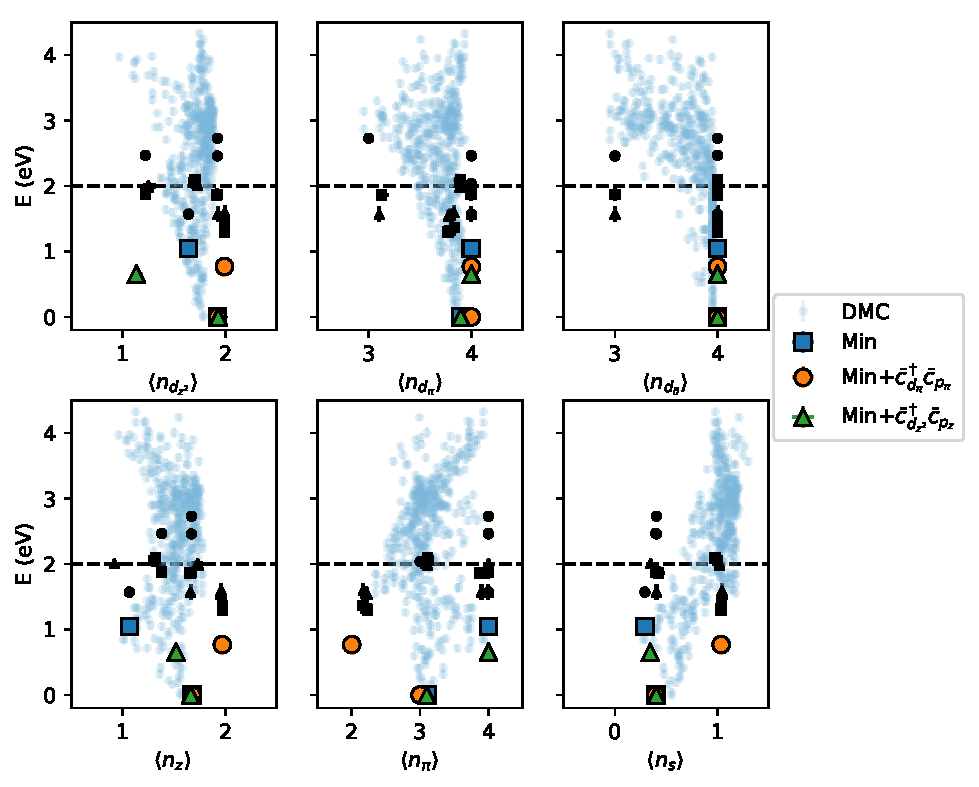
\includegraphics[width=0.45\textwidth]{figs/init_ed.pdf}
	}
	\qquad
	\subfigure[Collection of unique intruder states from our three potential models selected using a k-nearest neighbor approach with k = 5.]{	
		\label{fig:Intruder}
		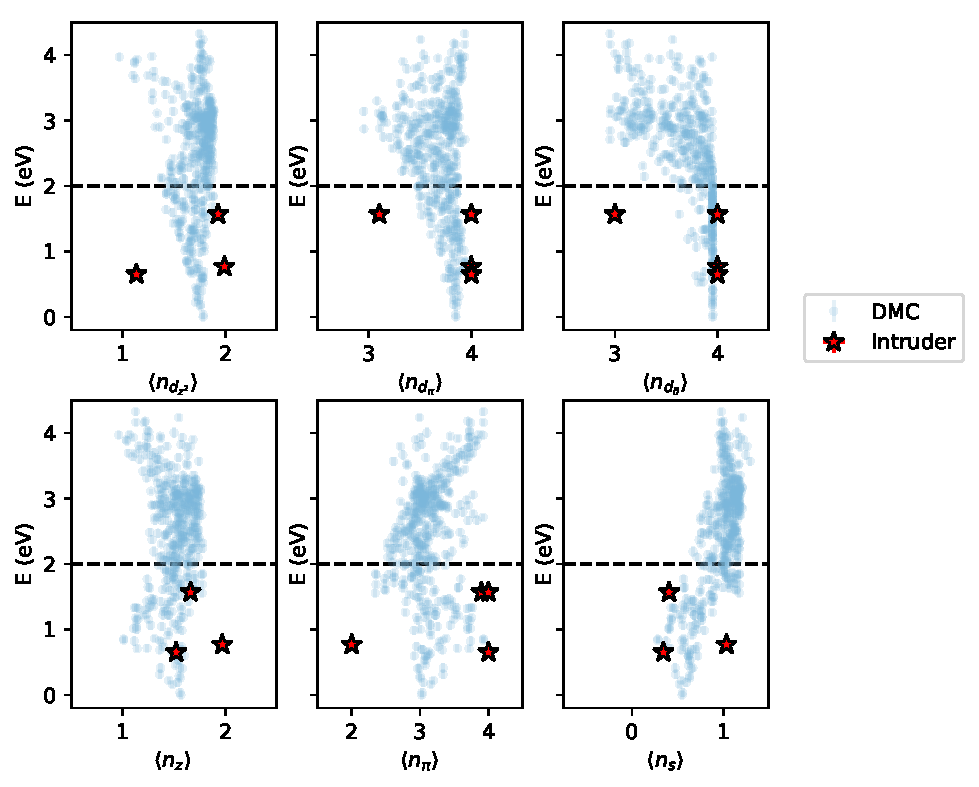
\includegraphics[width=0.45\textwidth]{figs/intruder.pdf}
	}
	\caption{Results of OLS fitting on sampled data and selected intruder states.}
\end{figure}

Given that our intruder states correspond to states within $\mathcal{LE}$ but outside our sample set, they must live within the span of the eigenstates which were excluded in our sampling scheme as described before.
This is evidenced by the fact that two of the intruder states correspond explicitly to excitations we could not access: Cu 3d$_{z^2} \rightarrow $ O 2p$_\pi$ and  Cu 3d$_\pi \rightarrow $ O 2p$_\pi$.
We can approximate these states by single rigid MO excitations above the UKS ground state, which results in states with a FN-DMC energy above 4eV.
Including a generous 2eV reduction in FN-DMC energy due to orbital relaxation, we estimate that these two states should lie at least 2eV in energy. 
Since all the other inaccessible eigenstates are double or higher order excitations, we assert a prior: intruder states should lie above 2eV in energy in our effective theories, enforced via an augmented cost function
\begin{equation}
\text{Cost} = \sum_{i} (E_\text{eff}[\Psi_i] - E_\text{ab}[\Psi_i])^2 + \lambda \sum_{p}\text{QHL}(2 - E_\text{eff}[\Psi_p]),\ \text{QHL}(x) = \Theta(x)x^2
\label{eq:cost}
\end{equation}
where $\lambda>0$ is a parameter which can be varied, QHL is a quadratic hinge loss, $\Theta$ is the Heaviside step function, the index $i$ is over our sampled states and $p$ over the selected intruder states.

\begin{figure}[H]
	\centering
	\subfigure[On the left, scores of the three candidate models at various $\lambda$ when fitting our effective theories using the cost function \eqref{eq:cost}. On the right we show predicted versus calculated energies for our low-energy sampled states for the minimal model fit at $\lambda = 20$.]{
	 	\label{fig:Prior}
		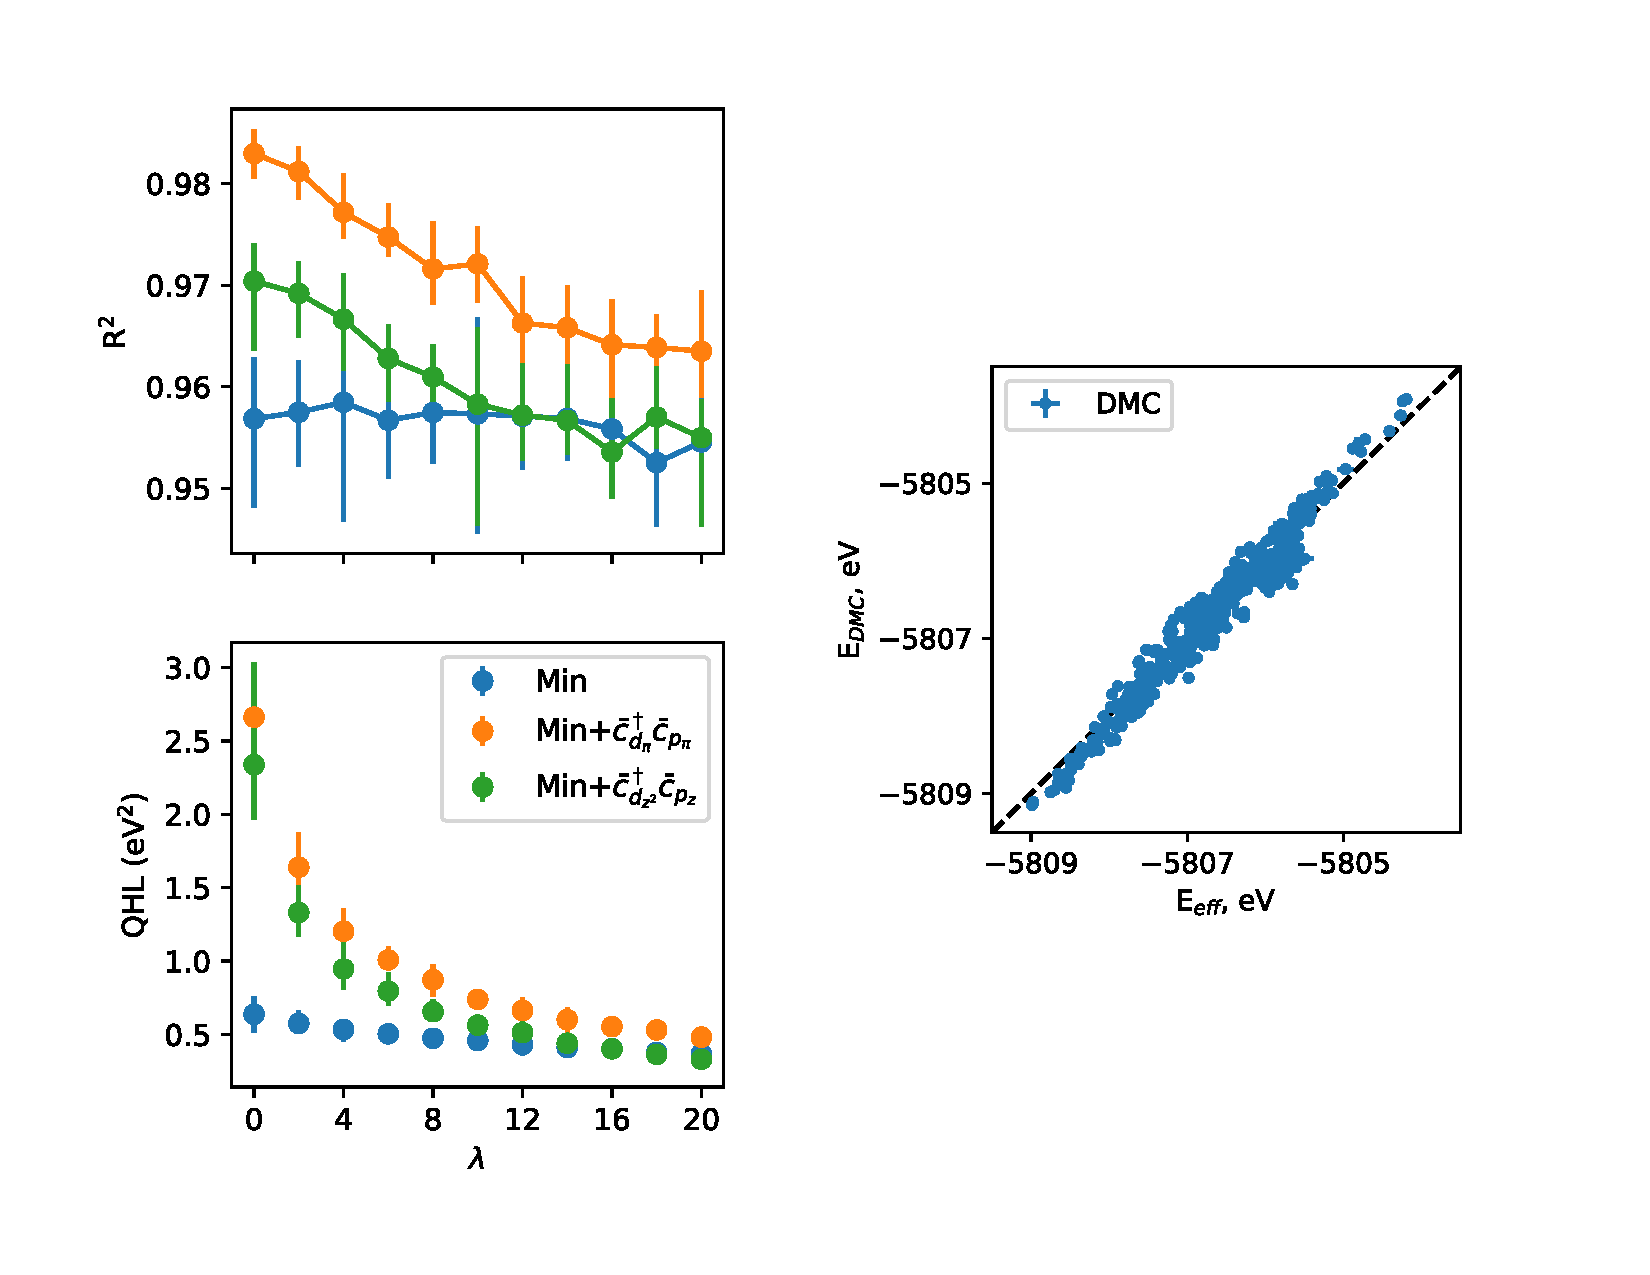
\includegraphics[width=0.45\textwidth]{figs/prior_and_regr.pdf}
	}
	\qquad
	\subfigure[Results of exact diagonalization showing the energies and properties of the first thirty eigenstates for three candidate models using linear regression with cost function \ref{eq:cost} and $\lambda = 20$. The ground state and first excited state are colored and have enlarged markers for clarity. Error bars are 95\% CI calculated by a bootstrap estimate.]{	
		\label{fig:FinalED}
		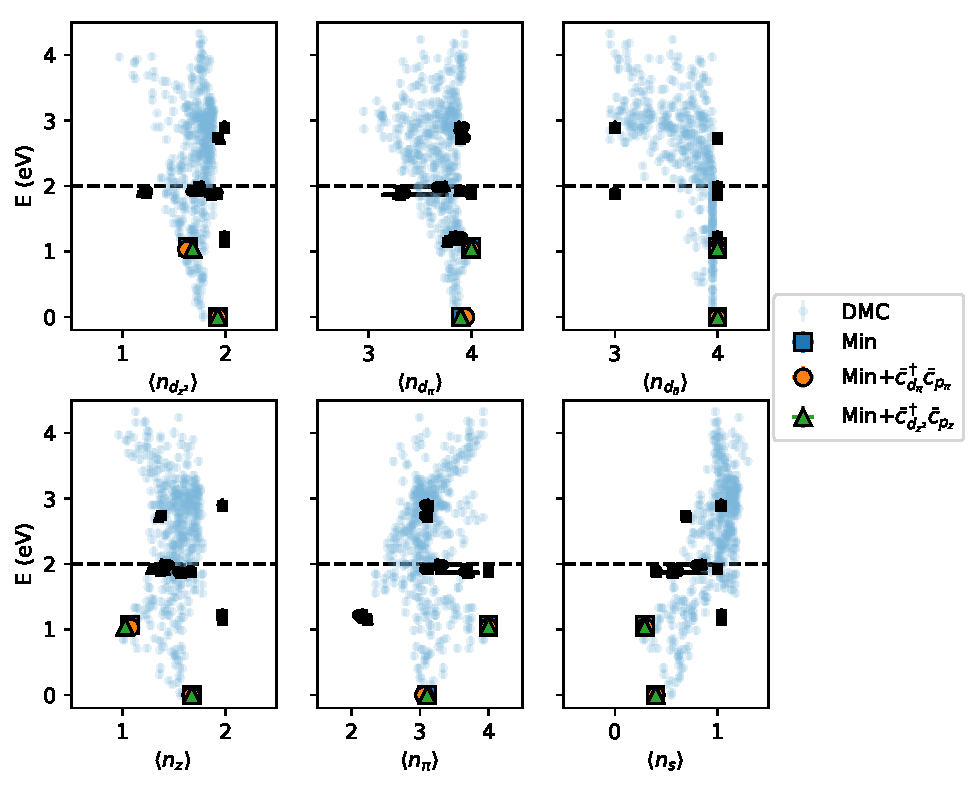
\includegraphics[width=0.45\textwidth]{figs/final_ed.pdf}
	}
	\caption{Results of linear regression using augmented cost function \eqref{eq:cost}.}
\end{figure}

Using our new cost function we find a set of models which accurately describe our sample data, have very similar spectra and eigenvectors to eachother and experiment, and do not contain intruder states below the 2eV prior. 
Shown in Figure \ref{fig:Prior} are the R$^2$ scores and QHL for the three candidate models fit at $\lambda \in [0,20]$. 
We believe that all three models at $\lambda = 20$ should be considered good models as they satisfy our prior and also explain our sample set accurately. 
Also shown are $E_\text{eff}, E_\text{ab}$ for our samples using the minimal model at $\lambda = 20$ to illustrate the high fit quality even with a large $\lambda$.
Figure \ref{fig:FinalED} presents the properties and eigenvalues of the lowest 30 eigenstates for the three fit models at $\lambda = 20$. 
The additional constraint from asserting a prior has seemingly caused a single effective theory to emerge from our set of candidate models.
This conclusion is verified by looking at the values of the fit parameters for our three models, presented in Table 1.
All occupation energies are relative to $\epsilon_{d_\delta}$.
In the doublet sector the ground and first excited state of any of the three models match experiment, as well as the block of states at 2eV corresponding to excitations out of the Cu 3d shell.
The lowest energy quartet states are at 1, 2eV respectively and are in line with the observation of a quartet state at 2eV in APES measurements.

\begin{table}[H]
\begin{center}
\begin{tabular}{l|lllll}
Model &$\epsilon_{d_{z^2}}$ & $\epsilon_{d_\pi}$ & $\epsilon_{4s}$ & $\epsilon_{p_\pi}$ & $\epsilon_{p_z}$ \\ \hline 
Min & 0.32(2)& 0.19(1)& 2.2(4)& 1.7(3)& 0.96(4)\\
Min $ +\ \bar{c}_{d_\pi}^\dagger \bar{c}_{p_\pi}$& 0.32(1)& 0.10(2)& 2.23(3)& 1.8(2)& 0.97(3)\\
Min $ +\ \bar{c}_{d_{z^2}}^\dagger \bar{c}_{p_z}$& 0.29(2)& 0.19(1)& 2.19(5)& 1.7(3)& 0.99(5)\\
\end{tabular} \\

\begin{tabular}{l|llllll}
Model &$t_\pi$ & $t_{dz}$ & $t_{sz}$ & $t_{ds}$ & $J_{sd}$ & $U_s$ \\ \hline 
Min &  -0.57(1)& 0.55(3)& 0.87(2)& 0.44(1)& -0.63(9)& 3.8(2)\\
Min $ +\ \bar{c}_{d_\pi}^\dagger \bar{c}_{p_\pi}$& -0.45(2)& 0.56(2)& 0.89(2)& 0.45(1)& -0.78(7)& 3.7(2)\\
Min $ +\ \bar{c}_{d_{z^2}}^\dagger \bar{c}_{p_z}$& -0.57(1)& 0.54(2)& 0.85(2)& 0.45(2)& -0.58(3)& 3.9(2)\\
\end{tabular} \\

\end{center}
Table 1: Parameters in eV for our three potential models when fit using \eqref{eq:cost} at $\lambda = 20$, energies relative to $\epsilon_{d_\delta} = 0$. Error bars are 95\% CI calculated using a bootstrap estimate.
\end{table}

\section{Proposed work}
My goal is to develop low-energy effective theories for the square lattice 1-band Hubbard model in order to map out the phases and transitions in the U-T space.
Recent attempts at solving this problem involve constructing single particle properties like densities of states using approximate numerical or effective theory techniques to classify different phases.
While instructive, reliance on single particle properties to identify phases instead of studying changes in the many-body Hilbert space and low-energy effective theory can lead to ambiguities regarding the nature of the phases.
I believe the DMD method can remove these ambiguities as the method explicitly involves studying changes in the low-energy Hilbert space and provides us with accurate many-body effective theories which can precisely differentiate different phases.

My first step would be to show whether the model supports more than one phase at T/t = 0 with respect to U, and if so what the features of these phases and the transition between them are.
I will investigate in particular the hypothesis that for $U/t<<1$ the model exhibits gapped Slater AFM behavior and for $U/t>>1$ Mott-Heisenberg behavior and whether the transition between them is a genuine phase transition or simply a crossover due to rearrangement of a few states.
To do so I will initially develop effective theories using DMD at two points U/t = 2, 12 and T/t = 0, allowing me to argue the existence or non-existence of multiple phases and investigate the properties of each phase.
I will follow by developing theories for various intermediate U in order to locate and study the transition between the two phases, if it exists, focusing on the hypothesis of a crossover U$^*/t\sim 4 - 5$ between the Slater and Mott-Heisenberg regimes.
Repeating this exercise for finite temperature I will build four more models at U/t = 2, 12 and T/t = 0.05, 0.20 to investigate the finite temperature phases at strong- and weak-coupling, in particular the claim of pseudogap and Fermi liquid phases at T/t = 0.05, 0.20 at weak coupling.
Filling in the U-T diagram will allow me to locate and study thermal transitions in the system. 
Building the T$>$0 effective theories will require special attention as they must satisfy the Mermin-Wagner theorem.

Similar to the case of the \textit{ab-initio} downfolding, I will need to construct low-energy spaces, sample the constructed spaces, build effective theories and respective bases, and fit candidate models.
I will begin from a starting point of highest control, namely for system sizes small enough where we can exactly diagonalize the Hubbard model.
In this case selecting $\mathcal{LE}$ can be done exactly as the span of some chosen $N$ lowest energy eigenstates. 
One can guarantee that the sample set fully encapsulates all low-energy degrees of freedom by sampling states parameterized as $|\Psi\rangle = \sum_{j=1}^N c_j |\Phi_j\rangle$ where $|\Phi_j\rangle$ are eigenstates of the Hubbard Hamiltonian.
Basis construction for the Hubbard Hamiltonian is also explicitly clear as any possible single particle basis we can use is just an orthogonal transformation of the basis the Hubbard model is defined on.
In order to include temperature into the mix one can work with the full model Hilbert space such that $\mathcal{LE} = \mathcal{H}$ but generate samples within the space using a Monte Carlo sampling method according to a Boltzmann probability distribution with variable parameter $\beta = 1/k_BT$, biasing the final model towards describing more accurately the energy functional on the states with highest weight.
Finite size extrapolation to the thermodynamic limit requires working with lattice sizes for which exact diagonalization is no longer feasible, and approximate methods like lattice variational Monte Carlo (VMC) will be employed to sample low-energy states as well as calculate energies and RDM elements.
In the weak and strong coupling regimes typical choices for varitional wave functions are non-interacting and Gutzwiller trial functions respectively, but other post-Gutzwiller and generalized Hartree Fock (GHF) trial functions have been shown to give accurate results in the moderate coupling regimes.
A rigorous prescription for finite size extrapolation specifically for the 1-band square lattice Hubbard model will be followed to extend our conclusions to the thermodynamic limit.

\begin{figure}[H]
\centering
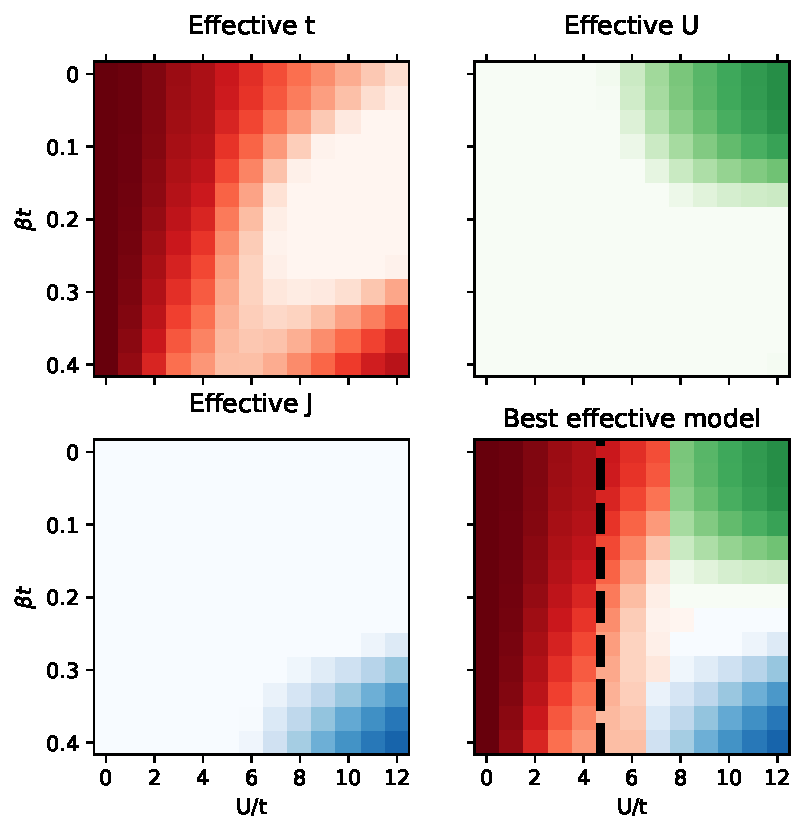
\includegraphics[width=0.6\linewidth]{figs/eff_eig_prelim.pdf}
\caption{Results of weighted single parameter model fits to the eigenstates of a Hubbard model for various U and temperature. Darker hues indicate a higher R$^2$ score. Vertical dashed line denotes the bulk Slater to Mott-Heisenberg transition U$^*$/t = 4.7 calculated in [ref].}
\label{fig:Hubbard}
\end{figure}	

I will conclude by showing some very preliminary results on model fitting for the half-filled, 2x2 square Hubbard model for U: 0 - 12 which put the outlined approach to model fitting with exact diagonalization at T$\geq 0$ into practice.
I started off by exactly diagonalizing each model, defining $\mathcal{LE} = \mathcal{H}$, and treating the full sample space as just the eigenstates of the model.
I then fit three single parameter models to the eigenstates: A) 
A "effective t" model $t_\text{eff} \sum_{\langle i, j \rangle, \sigma} c_{i\sigma}^\dagger c_{j\sigma} + h.c.$, B) An "effective U" model $U_\text{eff} \sum_{i} n_{i\uparrow} n_{i\downarrow}$, and C) An "effective J" model $J_\text{eff} \sum_{\langle i,j \rangle} \vec{S}_i \cdot \vec{S}_j$ using a weighted linear regression with weights $e^{-\beta E}$.
The basis for all of these operators are just the bare Hubbard Hamiltonian basis.
The weighted linear regression approximates the effect of generating samples using a Markov Chain Monte Carlo method with a Boltzmann distribution.
At low-temperatures there is a crossover between the weak coupling regime, best described by an effective t model, and the strong coupling regime, best described by an effective J model, around U$^*/t \sim 5$ providing some evidence of a Slater to Mott-Heisenberg transition.
In the crossover region T = 0 and U = 4 - 8 both models perform poorly and is a region of particular interest when developing our low-energy theories.
At high temperatures there is a crossover between the effective t and effective U models which can also be investigated.

\subsection{Proposed timeline}
I believe that developing effective theories for the half-filled Hubbard model should take 2 years. 
16 months should be spent on T = 0 calculations.
The first 8 months will be focused on exact diagonalization.
In this period, the first two months would be spent developing an efficient sampling scheme for $\mathcal{LE}$.
The following three months will be geared towards DMD for increasing system sizes from 2x2 to 4x4 lattices for U = 2, 12 in order to identify the existence of multiple zero temperature phases and will be primarily exploratory.
The next three months will be focused on studying intermediate U and the transition between the two phases, if they exist.
The following 8 months will be focused on finite size extrapolation.
The first two months here will be dedicated to extending our ED sampling scheme to VMC.
The following six months will involve extending our finite size results to the thermodynamic limit.
At the end of the first 16 months I should have a phase diagram at T = 0 with effective theories at various U.
The last 8 month chunk will be dedicated to the T $>$ 0 model fitting.
The first four months will be dedicated to exact diagonalization calculations and should be a relatively simple extension of the T = 0 model fitting with samples drawn according to an additional importance criteria $e^{-\beta E}$.
The last four months will be focused on extending our T = 0 VMC scheme to T $>$ 0 and conducting finite size extrapolation.
At the end of the 2 years I should have a phase diagram in the U - T space with effective theories at various values of U, T and an understanding of the phases and transitions between them.
\end{document}